% TO COMPILE:
% > pdflatex

\documentclass[11pt]{article}
\usepackage{enumitem}
\usepackage[english]{babel}
\usepackage[utf8]{inputenc}
\usepackage[colorlinks = true,
linkcolor = blue,
urlcolor  = blue]{hyperref}
\usepackage[a4paper,margin=1.5in]{geometry}
\usepackage{stackengine,graphicx}
\usepackage{fancyhdr}
% \usepackage{sectsty}
% \sectionfont{\noindent}
\setlength{\headheight}{15pt}
\usepackage{microtype}
\usepackage{times}
\usepackage{booktabs}
\usepackage{listings}
\usepackage{xcolor}
\lstdefinestyle{codestyle}{
	frame=single,
	basicstyle=\ttfamily\footnotesize,
	keywordstyle=\bfseries\color{magenta},
	commentstyle=\itshape\color{gray},
	stringstyle=\color{orange},
	numberstyle=\sffamily\scriptsize\color{gray},
	showspaces=false,
	showstringspaces=false,
	showtabs=false,
	tabsize=4,
	breakatwhitespace=false,
	breaklines=true,
	keepspaces=true,
	captionpos=b,
	numbers=left,
	numbersep=5pt}
\lstset{style=codestyle}

\pagestyle{fancy}
\fancyhf{}
\lhead{CS453}
\rhead{team 1}
\rfoot{\thepage}

\date{}

\title{Automated Refactoring\\for Pythonic Idioms\\with Differential Testing}

\begin{document}

\maketitle
\vspace{-2cm}
\thispagestyle{fancy}

\section{Introduction}
Python is widely used across various domains due to its rich libraries and flexible syntax. However, many developers struggle with writing \textbf{idiomatic} Python code, which can compromise readability, make maintenance more challenging, and sometimes even degrade performance. To address these issues, we have developed an \textbf{automated refactoring} technology. This technology transforms Python code into more \textbf{Pythonic} code, enhancing both readability and performance. To verify that the refactoring does not alter the functionality of the code, we have implemented \textbf{differential testing}. This method confirms that the code behaves the same before and after refactoring, thus securing the stability of the refactoring process. This report will discuss the necessity and effectiveness of this approach and examine how automated refactoring can improve the quality of Python code.\\

\section{Related Work}
\subsection{Making Python Code Idiomatic by Automatic Refactoring Non-idiomatic Python Code with Pythonic Idioms - Zhang et al. (2022)}
This study presented the first tool to automatically transform non-idiomatic Python code into idiomatic Python code. They analyzed 7,638 Python projects on GitHub, identifying \textbf{9 types} of 'Pythonic Idioms' that frequently occurred and could be converted from non-idiomatic code. Based on this, they defined specific syntactic patterns and developed a method of refactoring code through \textbf{abstract syntax tree (AST)} rewriting operations. Moreover, they applied these refactorings to actual code to verify the accuracy and usefulness of their tool. This research provides an essential foundation for our study, inspiring the design and implementation of our refactoring tool.\\
\subsection{A Peer Architecture for Lightweight Symbolic Execution - Alessandro Bruni, Tim Disney, Cormac Flanagan (2011)}
This study presents a lightweight, library-based approach to symbolic execution, leveraging the dynamic dispatch capabilities of object-oriented languages like Python. Instead of creating a new interpreter or compiler, their approach embeds a symbolic execution engine within the target program's process. This engine uses proxy objects to simulate symbolic values and track program execution paths. This provided a direction on how to perform symbolic execution for testing the functionality of functions.

\section{Approach}
\subsection{Automated Refactoring}
In this project, we laid the groundwork for the implementation of our refactoring tool by referencing the study of Zhang et al. and various literatures on Python idioms. Specifically, we selected \textbf{10 types} of refactorings that could enhance the performance and readability of Python code. These refactorings were implemented using the \textbf{Abstract Syntax Tree (AST)}, which provides a structural representation of source code. The AST is an ideal tool for systematically analyzing and modifying each element of the code. Through this, we developed a methodology that could automatically improve the code into a more Pythonic form.\\
Details of this part are all on \textbf{refactor.py}. For better understanding, we will write the (relevant code line) after the description of each part. For example, we inherited the NodeTransformer class and performed automated refactoring.\textbf{(413)}\\
When developing our automated refactoring tool, we assumed that the \textbf{source code is free of any errors}. This assumption allows us to focus solely on the refactoring process without the need to address or correct pre-existing code errors.\\ \\
(a) Collection Comprehension
\begin{lstlisting}[language=python]
# original
A=[]
for i in range(10):
    A.append(i)
for i in range(10):
    A.append(i*2)
# refactored
A = []
A += [i for i in range(10)]
A += [i * 2 for i in range(10)]
\end{lstlisting}
\textbf{Collection comprehension} transforms the declaration of \{lists, dictionaries and sets\} into a more Pythonic and efficient style. The node transformer class \textbf{CodeReplacer} calls the function \textbf{perform\_comprehension} for each function definition and module level to perform all possible comprehensions. In the refactored code, the list A is created and extended using list comprehensions, allowing multiple comprehensions to be combined effectively.
\\ \\
(b) Chaining Comparisons
\begin{lstlisting}[language=python]
# original
if d>e or (b>=c and d<=c and b<a and e>c) or e>10 and c>e:
    print("OK")
# refactored
if d > e or (e > c and a > b >= c >= d) or (c > e > 10):
\end{lstlisting}
\textbf {In} the refactored code, the original complex condition is broken down into more manageable parts by using Python's ability to chain comparisons directly. When \textbf{Visit\_If} is called, it invokes the function \textbf{transform\_chaining\_comparisons}, which checks all possible combinations and refactors them into the simplest equations possible.\\ \\
(c) Multiple Equality Comparisons
\begin{lstlisting}[language=python]
# original
name = "Joe"
if name == "Casey" or name == "Joe" or name == "Mike":
    print("yes")
# Refactored
name = 'Joe'
if name in ['Casey', 'Joe', 'Mike']:
    print('yes')
\end{lstlisting}
\textbf{Multiple Equality Comparisons} code auto-refactoring simplifies the process of comparing a variable against multiple values. The refactored version replaces these with a membership test using the 'in' keyword, checking if the variable is within a list of values. The node transformer class \textbf{CodeReplacer} applies the function \textbf{transform\_equality\_comparisons} for every \textbf{Visit\_If}. \\ \\
(d) Merge Append
\begin{lstlisting}[language=python]
# original
A = []
A.append(1)
A.append(2)
A.pop()
A.append(3)
A.append(4)
# Refactored
A = []
A += [1, 2]
A.pop()
A += [3, 4]
\end{lstlisting}
\textbf{Merge multiple append} optimizes the code by combining consecutive append calls into a single operation using list addition. The function \textbf{transform\_list\_appends}, which is responsible for it, checks every append call within a module and function, and merges them into a single \textbf{augAssign} when more than two appends are detected, utilizing AST. The original sequence of \textbf{A.append} calls is replaced by \textbf{A += [1, 2]} and \textbf{A += [3, 4]}, consolidating the append operations while maintaining the same functionality. \\ \\
(e) Test Empty Collection
\begin{lstlisting}[language=python]
# original
if A==[]:
    print(1)
elif B!=():
    print(2)
# refactored
if not A:
    print(1)
elif B:
    print(2)
\end{lstlisting}
\textbf{Test collection} changes a comparison with Eq(==) or NEq(!=) which one side is empty collections (list, tuple, dictionary) or empty string to a form without a comparison. Therefore, we overwrite \textbf{visit\_Compare}, and change the content of the node to \#refactored in code snippet when the above conditions are satisfied.(7)\\ \\
(f) Merge If
\begin{lstlisting}[language=python]
# original
if A:
    if B:
		if C:
        	print(2)
		else:
			print(3)
# refactored
if A and B:
	if C:
    	print(2)
	else:
		print(3)
\end{lstlisting}
\textbf{Merge If} combines multiple If statements into one using the and operator when they appear consecutively. Therefore, we overwrite \textbf{visit\_If} and change the content of the node to \#refactored in code snippet when the above conditions are satisfied.\\
However, it is crucial to consider cases where the if statement \textbf{appears with else} together, which would make merging inappropriate. For example, consider the lines 2, 3 and 5 of the code snippet. To handle this case, when a If node has \textbf{node.orelse}, we don't apply the merge.(30)\\
Also, to merge 3 or more mergeable If statements, we first implement \textbf{generic\_visit}.(459)\\ \\
(g) If Expression
\begin{lstlisting}[language=python]
# original
if A:
    x=1
else:
    x=2
if A:
    print(1)
else:
    print(2)
# refactored
x = 1 if A else 2
print(1 if A else 2)
\end{lstlisting}
\textbf{If Expression} changes a general If-else syntax to IfExpression when the contents of the If-else are \textbf{different only in value and perform the same function (assignment, print)}. Therefore, we overwrite \textbf{visit\_If} and change the content of the node when the above conditions are satisfied.(47)\\ \\
(h) to Enumerate
\begin{lstlisting}[language=python]
# original
for i in range(len(players)):
    print(i, players[i])
    print(players[i-1])
    players[i] = 1
# refactored
for i, item in enumerate(players):
    print(i, item)
    print(players[i - 1])
    players[i] = 1
\end{lstlisting}
\textbf{to Enumerate} always changes the form of the range (len(list or tuple)) in the for statement to enumerate (list or tuple). Therefore, we overwrite \textbf{visit\_For}.(67)\\
For convenience, we unify the variable to store the element of the list as \textbf{item}. In addition, by overwriting \textbf{visit\_Subscript}, we use \textbf{item} instead of the list \textbf{element by using current index} inside the for statement in the source code.(87) To implement this function, we defined a dictionary called \textbf{self.toItem}.(415) At the beginning of the visit of the for statement, add \textbf{(list name):(index)} to the self.toItem(77), and pop when all the visit of the for statement is over.(430)\\
However, it is crucial to consider cases where accessing an element of an index \textbf{different from the current index} of the list or assigning a new value \textbf{to the current index element} of the list. For example, the lines 9 and 10 in code snippet. To handle these cases, we check that each node satisfies the above state in visit\_Assign and visit\_Subscript, and if so, we did not proceed with the change to item.(89, 439)\\ \\
(i) Return Boolean Statement
\begin{lstlisting}[language=python]
# original
def func(A):
    if A:
        return True
    else:
        return False
# refactored
def func(A):
    return A
\end{lstlisting}
\textbf{Return Boolean Statement} is possible only when returning a Boolean value with different internal branches with if-else statement. Therefore, we overwrite \textbf{visit\_If}, and change the content of the node when the above conditions are satisfied.(104)\\ \\
(j) Multiple Assign
\begin{lstlisting}[language=python]
# original
a=2
b=3
c=4
d=c+1
# refactored
a,b,c=2,3,4
d=c+1
\end{lstlisting}
\textbf{Multiple assistance} can occur in any part of the Python code. The strategy involves modifying the \textbf{generic\_visit} method to find out all nodes that contain a 'body' attribute, and \textbf{traverse node.body} which includes the potential for multiple assignments.(417)\\
However, it is crucial to consider cases where variables from previous assignments are used in subsequent ones, which would make merging inappropriate. For example, consider the \textbf{c} and \textbf{d} on the lines 4 and 5 of a code snippet. To handle this case, we apply always storing the previous element and comparing it with the current element while traverse all node.body.(147)\\

\subsection{Differential Testing}
The purpose of refactoring is to improve the structure of the code, enhancing readability and performance, without changing the functional behavior of the code. If the refactored code behaves differently from the original code, it cannot be considered correctly refactored. Therefore, it is crucial to ensure that the refactored Python source code operates identically to the original code. In this section, we perform differential testing to verify this, using two methods to confirm that the refactored code operates the same as the original one. \\ \\

(a) Function Test\\ \\
The first method is to test whether the functions implemented in the code produce the same return values. Since the behavior of a function depends on the input parameters, a variety of values should be used as input parameters. We used symbolic execution to obtain the input parameters that directly execute the modified parts. The purpose of the function test is to verify whehter the return values of the functions differ by generating all possible combinations of input parameters for every conditional statement and branch within the code through symbolic execution, thus covering as much of the code as possible. If the return values differ for a specific input, it indicates that the refactoring was not performed correctly. \\
Symbolic execution involves executing the target program not with concrete test inputs but with symbolic proxy objects set as input parameters. These proxy objects allow the symbolic engine to track and analyze the execution flow of the program. In this process, it is possible to observe how the program manipulates the input parameters and how these manipulations affect the rest of the program.
Unlike many other programming languages, Python does not provide type hints normally, making it difficult to determine the types of input parameters based solely on the information provided by the function. In order to solve this problem, we created an 'AnyProxy' class and used it as the input parameters for the functions. This class helps to generalize input types initially, and then, based on the behavior of the program, it differentiates these inputs into specific types for further processing.

\begin{center}
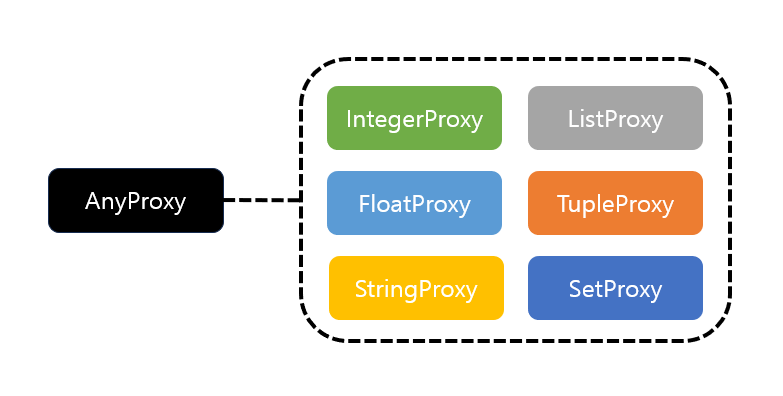
\includegraphics[width = 10cm]{Anyproxy_to_proxies.PNG}

{Figure 1. The proxy classes differentiated from AnyProxy class}
\end{center}

\pagebreak

Figure 1 illustrates how the AnyProxy class we implemented branches into specific classes. AnyProxy is initially set as the input parameters of a function and, during the execution of program, differentiates into specific types of proxy objects through various operations and method calls. The AnyProxy object differentiates into a specific type of proxy object in the following situations. \\ \\
1. Operation with a specific type: When the AnyProxy object performs an operation with data of a specific type, it transforms into a proxy object corresponding to that type. For example, if an AnyProxy object performs an addition operation with an int type, it differentiates into an IntegerProxy object. \\

\begin{lstlisting}[language=python]
def get_proxy(self, other):
        if isinstance(other, (int, IntegerProxy)):
            return IntegerProxy(Int(self.name)), other
        elif isinstance(other, (float, FloatProxy)):
            return FloatProxy(Real(self.name)), other
        elif isinstance(other, (str, StringProxy)):
            return StringProxy(String(self.name)), other
        ...
\end{lstlisting}

2. Specific method call: When the AnyProxy object encounters a method that is unique to a specific type, it transforms into a proxy object for that type. For example, it the AnyProxy object calls 'append' method, which is unique to the list type, it differentiates into a ListProxy object. \\

\begin{lstlisting}[language=python]
def __getitem__(self, index):
        if isinstance(index, AnyProxy):
            index = IntegerProxy(Int(index.name))
        return ListProxy(IntVector(self.name, self.length), self.name).__getitem__(index)
\end{lstlisting}


(b) Execution Test\\ \\

The second method involves verifying that the refactored Python code behaves identically to the original Python code by directly executing both codes and comparing their standard stream outputs. This is achieved using the Python 'subprocess' module to compare the values output to 'stderr' and 'stdout'. If the results differ, it indicates that there were some problems during the refactoring process, and an error is returned. \\
\begin{lstlisting}[language=python]
def test_refactored_code(original_path, test_path):
    cur_dir = os.getcwd()
    test_case_path = os.path.dirname(original_path)
    ori_file_name = os.path.basename(original_path)
    test_file_name = os.path.basename(test_path)
    os.chdir(test_case_path)
    cmd1 = ['python', ori_file_name]
    result1 = subprocess.run(cmd1, capture_output=True, text=True)
    cmd2 = ['python', test_file_name]
    result2 = subprocess.run(cmd2, capture_output=True, text=True)

    os.chdir(cur_dir)
    try:
        assert result1.stdout == result2.stdout
        assert result1.stderr == result2.stderr
    except Exception as e:
        print("Error while testing stdout and stderr", e)
\end{lstlisting}

\section{Evaluation}
\subsection{Efficiency}
...\\

\subsection{Readability?}
...\\

\subsection{Differential Testing}
...\\

\section{Threat to Validity}
\subsection{Handling Corner Cases in Automated Refactoring}
One of the threats to validity in the development of our automated refactoring tool is the \textbf{potential failure to perfectly handle specific corner cases}. Although we attempted to cover all conceivable counterexamples theoretically, it is practically challenging to anticipate every scenario due to the limits of imagination. To overcome this limitation, we adopted an approach of applying automated refactoring to \textbf{existing Python codes}, examining the outcomes to identify and modify counterexamples. In particular, we utilized various code examples from programming problem platforms like \textbf{Baekjoon} to assess the applicability and usefulness of our tool. This process has allowed us to enhance the robustness of our refactoring tool in handling diverse real-world use cases.\\

\subsection{Covering other type of inputs}
In the function testing part of the differential testing, we did not cover any type existed in Python. This is because there are limitations in the Z3 solver and challenges in type inference system of Python. The Z3 solver, while powerful, has limitations in handling complex user-defined types. Additionally, Python's dynamic typing and lack of type hints complicate accurate type inference. Therefore we were unable to implement code that covers all types. We can only create test cases for certain function which get specialized input parameters. These constraints may affect the generalizing. However, we expect that, with more cases' testing, the range of covering can be improved. \\

\section{Discussion \& Conclusion}
...\\


\end{document}